% Parte 2 del TP2 (ING560): borrador de presentación, 8 minutos de exposición.
% Compilar desde esta carpeta:  latexmk -pdf presentacion.tex          (diapositivas)
%                               latexmk -pdf presentacion_notas.tex    (con notas para quien expone)
% Las figuras se generan con codigo/figuras.py en ../resultados/figuras/.
\documentclass[aspectratio=169, 10pt]{beamer}

\usepackage[utf8]{inputenc}
\usepackage[spanish]{babel}
\usepackage{amsmath, amsfonts, amssymb}
\usepackage{booktabs}
\usepackage{graphicx}
\usepackage{tikz}
\usetikzlibrary{positioning, arrows.meta, fit}
\usepackage{hyperref}
\graphicspath{{../resultados/figuras/}}

\ifdefined\conNotas
  \usepackage{pgfpages}
  \setbeameroption{show notes on second screen=right}
\fi
\setbeamertemplate{note page}{\footnotesize\insertnote}

% --- Estilo de la presentación anterior del curso (Lin_Opti/presentacion.tex) ---
\usetheme{Madrid}
\useinnertheme{rectangles}
\definecolor{NavyDark}{RGB}{15, 34, 64}
\definecolor{SlateBlue}{RGB}{41, 74, 110}
\definecolor{AccentTeal}{RGB}{20, 140, 130}
\definecolor{SoftGray}{RGB}{245, 247, 250}
\definecolor{Charcoal}{RGB}{40, 40, 40}
\definecolor{AlertRed}{RGB}{190, 40, 40}
\setbeamercolor{palette primary}{bg=NavyDark, fg=white}
\setbeamercolor{palette secondary}{bg=SlateBlue, fg=white}
\setbeamercolor{palette tertiary}{bg=NavyDark, fg=white}
\setbeamercolor{structure}{fg=NavyDark}
\setbeamercolor{frametitle}{bg=NavyDark, fg=white}
\setbeamercolor{title}{bg=NavyDark, fg=white}
\setbeamercolor{block title}{bg=SlateBlue, fg=white}
\setbeamercolor{block body}{bg=SoftGray, fg=Charcoal}
\setbeamercolor{block title alerted}{bg=AlertRed, fg=white}
\setbeamercolor{block body alerted}{bg=SoftGray, fg=Charcoal}
\setbeamercolor{block title example}{bg=AccentTeal, fg=white}
\setbeamercolor{block body example}{bg=SoftGray, fg=Charcoal}
\setbeamertemplate{navigation symbols}{}
\setbeamertemplate{footline}[frame number]

% Marcador visible para lo que debe completar el grupo.
\newcommand{\pendiente}[1]{\textcolor{AlertRed}{\textbf{[#1]}}}
\newcommand{\archivo}[1]{{\scriptsize\texttt{#1}}}

\title[Spam en SMS con un transformer pequeño]{\textbf{¿Cuánto aporta la atención para detectar spam en SMS?}}
\subtitle{Un transformer pequeño entrenado desde cero y una comparación controlada de optimizadores}
\author[\pendiente{Grupo}]{\pendiente{Integrantes del grupo}}
\institute[UAI]{ING560 — Álgebra Lineal y Optimización para Data Science\\
  \vspace{0.2cm}\textit{Trabajo Práctico 2, Parte 2}}
\date{\pendiente{Fecha de la presentación}}

\begin{document}

% =============================================================================
\begin{frame}
  \titlepage
\end{frame}
\note{
  \textbf{Portada (10 s).} Presentar al grupo y la pregunta: ¿un transformer pequeño, entrenado
  desde cero en CPU, supera a un modelo lineal clásico para detectar spam? El foco es cómo se
  entrena y cómo cambia el resultado con el optimizador y la tasa de aprendizaje.
}

% =============================================================================
% 1. PROBLEMA, DATOS Y OBJETIVO (1 min)
% =============================================================================
\begin{frame}{Problema, datos y objetivo}
  \small
  \begin{columns}[T]
    \begin{column}{0.49\textwidth}
      \begin{block}{Objetivo}
        Clasificar un SMS como \textbf{spam} o \textbf{ham} (legítimo) según su texto.
        Métrica: \textbf{F1 de la clase spam}; decir siempre «ham» ya da 87,6\,\% de exactitud.
      \end{block}
      \vspace{0.1cm}
      \begin{block}{Datos: SMS Spam Collection}
        \begin{itemize}
          \item Almeida y Gómez Hidalgo (2011), UCI ML Repository.
          \item Licencia \textbf{CC BY 4.0}; descarga directa, sin cuenta.
          \item 5574 SMS en inglés: etiqueta y texto; 13\,\% spam.
          \item Cortos: mediana 16 tokens, percentil 99 $\approx$ 65.
        \end{itemize}
      \end{block}
    \end{column}
    \begin{column}{0.49\textwidth}
      \begin{block}{Partición sin filtraciones}
        \begin{itemize}
          \item Se quitan 414 SMS repetidos $\Rightarrow$ 5160 únicos.
          \item Estratificada 70/15/15 (semilla 2026):\\ 3612 / 774 / 774 SMS, con 449 / 96 / 97 spam.
          \item Vocabulario (3184 tokens) y TF-IDF: \textbf{solo entrenamiento}.
          \item Prueba: un script aparte, una vez, al final.
        \end{itemize}
      \end{block}
      \vspace{0.1cm}
      \begin{exampleblock}{¿Por qué un transformer?}
        La señal está en combinaciones de palabras («call now», «txt STOP to»); la atención
        relaciona cada token con todos los demás del mensaje.
      \end{exampleblock}
    \end{column}
  \end{columns}
  \vfill
  \archivo{datos/fuente.json, datos/resumen\_datos.json, codigo/preparar\_datos.py}
\end{frame}
\note{
  \textbf{1 min.} Qué se predice (spam/ham), de dónde salen los datos y su licencia.
  Recalcar las dos decisiones contra filtraciones: quitar los 414 duplicados antes de
  separar y ajustar vocabulario y TF-IDF solo con entrenamiento. Explicar por qué se usa F1:
  hay 12,4\,\% de spam y el predictor constante ya tiene 87,6\,\% de exactitud.
  Pregunta probable: ¿por qué 64 tokens? Cubre el 99\,\% de los mensajes; solo 37 de 3612 se truncan.
}

% =============================================================================
% 2. ARQUITECTURA Y PESOS ENTRENABLES (1 min)
% =============================================================================
\begin{frame}{Arquitectura y parámetros entrenables}
  \begin{columns}[T]
    \begin{column}{0.50\textwidth}
      \centering
      \begin{tikzpicture}[
          caja/.style={draw=SlateBlue, fill=SoftGray, rounded corners=2pt, minimum width=4.6cm,
                       minimum height=0.48cm, font=\scriptsize, align=center},
          flecha/.style={-{Stealth[length=4pt]}, SlateBlue, thick},
          node distance=0.17cm]
        \node[caja] (tok) {SMS $\to$ hasta 64 tokens (índices del vocabulario)};
        \node[caja, below=of tok] (emb) {$X = E_{\text{tok}}[\text{token}] + E_{\text{pos}}[\text{posición}] \in \mathbb{R}^{n\times 64}$};
        \node[caja, below=0.32cm of emb, fill=white] (att) {LayerNorm $\to$ atención de 4 cabezas ($d_k=16$) $\to +X$};
        \node[caja, below=of att, fill=white] (ffn) {LayerNorm $\to$ FFN $64\to128\to64$ (ReLU) $\to +X$};
        \node[draw=AccentTeal, thick, rounded corners=3pt, fit=(att)(ffn), inner sep=4pt,
              label={[font=\scriptsize\bfseries, text=AccentTeal]right:$\times 2$}] (bloque) {};
        \node[caja, below=0.32cm of ffn] (pool) {LayerNorm $\to$ promedio de los tokens reales $z\in\mathbb{R}^{64}$};
        \node[caja, below=of pool] (sal) {$P(\text{spam}) = \sigma(w^\top z + b)$};
        \draw[flecha] (tok) -- (emb);
        \draw[flecha] (emb) -- (bloque);
        \draw[flecha] (bloque) -- (pool);
        \draw[flecha] (pool) -- (sal);
      \end{tikzpicture}\\[4pt]
      {\scriptsize Cada cabeza: $Q=XW_Q$, $K=XW_K$, $V=XW_V$,
       $A=\mathrm{softmax}\big(QK^\top/\sqrt{16} + M\big)$, $H=AV$;\\
       $M_{ij}=-\infty$ si el token $j$ es relleno.}
    \end{column}
    \begin{column}{0.47\textwidth}
      \scriptsize
      \begin{tabular}{@{}lr@{}}
        \toprule
        \textbf{Componente} & \textbf{Parámetros} \\
        \midrule
        Embeddings de token ($3184 \times 64$) & 203\,776 \\
        Embeddings de posición ($64 \times 64$) & 4\,096 \\
        Atención $W_Q, W_K, W_V, W_O$ (+ sesgo), 2 capas & 32\,896 \\
        FFN $64\to128\to64$, 2 capas & 33\,152 \\
        LayerNorm (5 de ellas, $\gamma$ y $\beta$) & 640 \\
        Clasificador $w, b$ & 65 \\
        \midrule
        \textbf{Total entrenable} (contado con código) & \textbf{274\,625} \\
        \bottomrule
      \end{tabular}\\[6pt]
      \begin{itemize}
        \item El 74\,\% de los pesos son embeddings de token: el vocabulario manda.
        \item Dentro de los máximos de la sección 4.2: 2 capas, $d=64$, 4 cabezas,
              $n\le 64$, $<1$ M de parámetros, 3612 ejemplos.
        \item Una corrida de 250 pasos: 13--24 s en 2 CPU; las 21 corridas, 4,3 min.
      \end{itemize}
      \vfill
      \archivo{codigo/comun.py, resultados/parametros\_transformer.csv}
    \end{column}
  \end{columns}
\end{frame}
\note{
  \textbf{1 min.} Recorrer el diagrama de arriba abajo. La atención está escrita con
  operaciones explícitas (las mismas $Q,K,V,S,A,H$ de la Parte 1), con una máscara para no
  atender al relleno. Diferenciar pesos entrenables ($E$, $W_Q$, $W_K$, $W_V$, $W_O$, FFN,
  LayerNorm, $w$, $b$) de cantidades calculadas ($Q,K,V,A,H$). La cuenta sale de
  \texttt{parametros\_transformer.csv}: 274\,625. Detalle si preguntan: la fila del token de
  relleno (64 pesos) nunca recibe gradiente.
}

% =============================================================================
% 3. ENTRENAMIENTO Y OPTIMIZACIÓN (2,5 min, primera parte)
% =============================================================================
\begin{frame}{Entrenamiento y diseño de la comparación}
  \small
  \begin{columns}[T]
    \begin{column}{0.44\textwidth}
      \textbf{Pérdida:} entropía cruzada binaria, lote $B=32$
      \[ \mathcal{L} = -\tfrac{1}{B}\textstyle\sum_i \big[y_i\log\sigma(z_i) + (1-y_i)\log(1-\sigma(z_i))\big] \]
      \textbf{SGD con momento:} $v \leftarrow 0{,}9\,v+g$, \ $\theta \leftarrow \theta-\eta\,v$\\
      \textbf{AdamW:} $\theta \leftarrow \theta-\eta\big(\hat m/(\sqrt{\hat v}+\epsilon)+0{,}01\,\theta\big)$
      \begin{block}{Constante}
        Modelo, datos, pesos iniciales y orden de lotes (misma semilla), \textbf{250 pasos}
        (2,2 épocas), $\eta$ constante, sin recorte.
      \end{block}
      \begin{block}{Varía: 6 configuraciones $\times$ 3 semillas}
        \textbf{A.} AdamW, $\eta \in \{10^{-4}, 10^{-3}, 10^{-2}\}$\\
        \textbf{B.} SGD con momento, $\eta \in \{10^{-2}, 10^{-1}, 1\}$\\
        \textbf{C.} Normas del gradiente y del paso\\
        Se elige por F1 medio en validación.
      \end{block}
    \end{column}
    \begin{column}{0.54\textwidth}
      \centering
      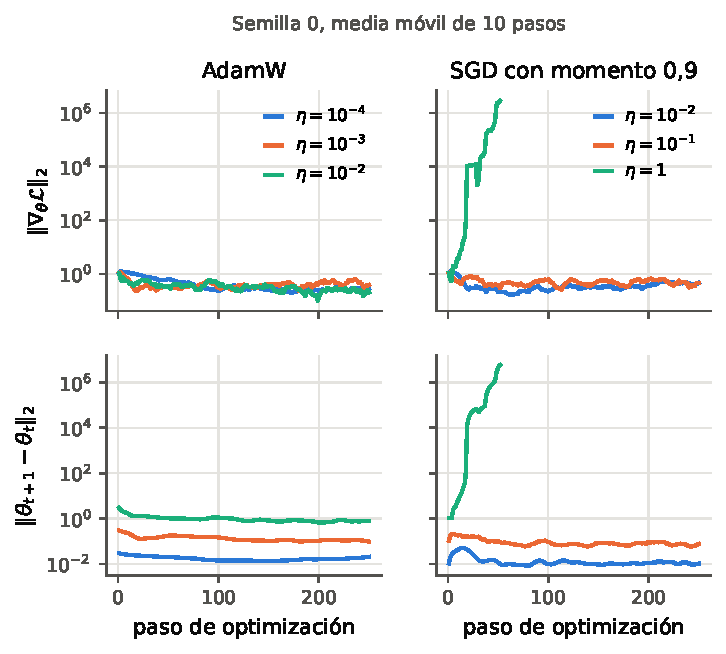
\includegraphics[width=\linewidth,height=0.78\textheight,keepaspectratio]{normas_gradiente}\\
      \archivo{resultados/registro\_pasos.csv}
    \end{column}
  \end{columns}
\end{frame}
\note{
  \textbf{1 min 15 s.} Pérdida y optimizadores en una frase cada uno. Insistir en el control: con
  la misma semilla todas las configuraciones parten de los mismos pesos y ven los mismos lotes;
  solo cambia el optimizador o $\eta$. Lectura de la figura (experimento C): la norma del gradiente
  es parecida en todas las corridas estables (mediana 0,2--0,4 entre los pasos 100 y 250), pero el
  tamaño del paso no: en AdamW crece con $\eta$ (0,016; 0,11; 0,79) porque normaliza cada
  coordenada; en SGD es $\eta$ por el gradiente acumulado. Con SGD y $\eta=1$ hay un círculo
  vicioso: paso grande $\Rightarrow$ gradiente grande $\Rightarrow$ paso mayor, más de $10^7$ en
  las 3 semillas, hasta una pérdida no finita. AdamW con $\eta=10^{-2}$ se mueve unas 10 veces más por paso que el mejor SGD.
  Fuente: \texttt{registro\_pasos.csv} y \texttt{figuras/resumen\_normas.csv}.
}

% =============================================================================
% 4. CURVAS DE LOS EXPERIMENTOS A Y B (2,5 min, segunda parte)
% =============================================================================
\begin{frame}{Experimentos A y B: velocidad y estabilidad}
  \begin{columns}[T]
    \begin{column}{0.58\textwidth}
      \centering
      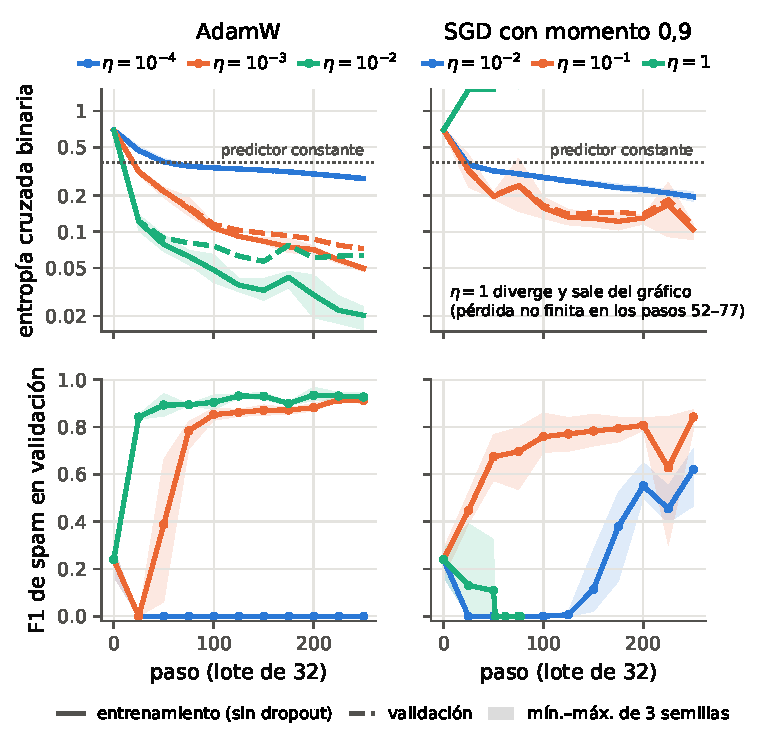
\includegraphics[width=\linewidth,height=0.77\textheight,keepaspectratio]{curvas_entrenamiento}\\
      \archivo{resultados/registro\_evaluacion.csv}
    \end{column}
    \begin{column}{0.41\textwidth}
      \footnotesize
      \textbf{A. Tasa con AdamW}
      \begin{itemize}
        \item $10^{-4}$: la pérdida baja del predictor constante (0,375 $\to$ 0,27), pero ningún
              SMS llega a $P>0{,}5$: F1 = 0. Aprende, pero lento.
        \item $10^{-3}$: estable; en el paso 250 la validación aún baja (0,072).
        \item $10^{-2}$: F1 0,84 en 25 pasos. Desde el paso 150 la validación se estanca
              (0,057 $\to$ 0,064) mientras entrenamiento baja (0,033 $\to$ 0,020): sobreajuste.
      \end{itemize}
      \textbf{B. SGD con momento}
      \begin{itemize}
        \item $10^{-2}$: F1 despega recién tras el paso 125.
        \item $10^{-1}$: el mejor SGD, pero ruidoso.
        \item $1$: diverge en las 3 semillas (pasos 52--77).
      \end{itemize}
    \end{column}
  \end{columns}
\end{frame}
\note{
  \textbf{1 min 15 s.} Leer primero la fila de arriba (pérdida, escala log) y después F1.
  Mensaje: con el mismo presupuesto, $\eta$ decide si el modelo no alcanza a aprender
  ($10^{-4}$), aprende bien ($10^{-3}$, $10^{-2}$) o diverge (SGD con 1). La línea punteada es la
  pérdida de predecir siempre 12,4\,\% de spam: bajo ella el modelo ya usa el texto, aunque F1
  siga en 0 porque ninguna probabilidad cruza 0,5. Las configuraciones lentas pasan por F1 = 0:
  primero aprenden la proporción de clases y después las palabras. Las bandas son mínimo y
  máximo entre semillas: SGD varía mucho más entre semillas que AdamW.
}

% =============================================================================
% 5. COMPARACIONES Y MÉTRICAS (2,5 min)
% =============================================================================
\begin{frame}{Selección en validación (AdamW, $\eta=10^{-2}$) y evaluación final en prueba}
  \begin{columns}[T]
    \begin{column}{0.50\textwidth}
      \centering
      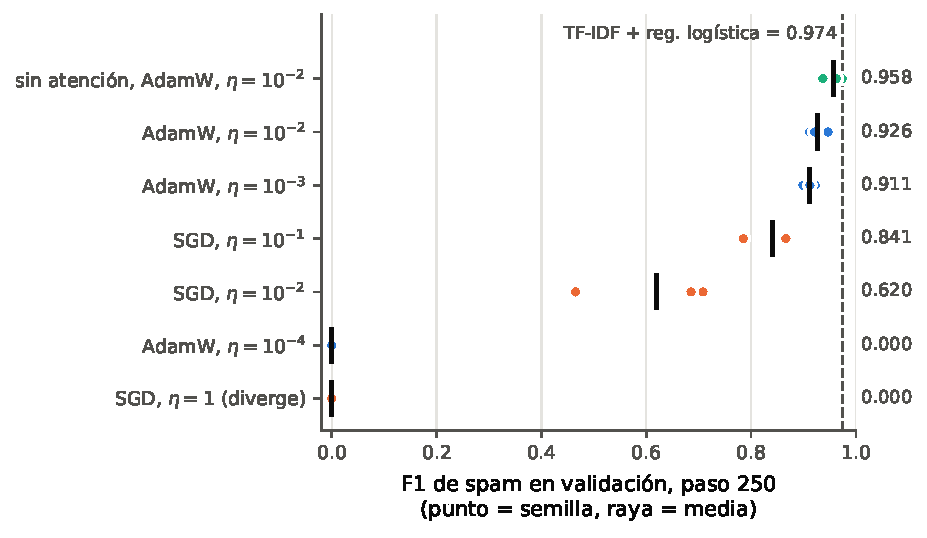
\includegraphics[width=\linewidth,height=0.8\textheight,keepaspectratio]{comparacion_validacion}\\[2pt]
      \archivo{resultados/resumen\_configuraciones.csv, resultados/seleccion.json}
    \end{column}
    \begin{column}{0.48\textwidth}
      \scriptsize
      \textbf{Prueba} (774 SMS, 97 spam; umbral 0,5; transformer: media $\pm$ desv. de 3 semillas)\\[2pt]
      \begin{tabular}{@{}lccc@{}}
        \toprule
        & \textbf{Transformer} & \textbf{TF-IDF + RL} & \textbf{Mayoritaria} \\
        \midrule
        F1 spam        & 0,893 $\pm$ 0,006 & \textbf{0,931} & 0 \\
        Precisión      & 0,948 $\pm$ 0,038 & 0,957 & -- \\
        Exhaustividad  & 0,845 $\pm$ 0,027 & \textbf{0,907} & 0 \\
        Exactitud      & 0,975 $\pm$ 0,002 & 0,983 & 0,875 \\
        Entropía cruz. & 0,100 $\pm$ 0,006 & 0,084 & -- \\
        Parámetros     & 274\,625 & 41\,924 & -- \\
        \bottomrule
      \end{tabular}\\[4pt]
      \begin{itemize}
        \item \textbf{Resultado negativo:} el transformer no supera a la referencia. La diferencia
              pareada de F1 (bootstrap 95\,\%) excluye el 0 en 2 de 3 semillas.
        \item Pierde en exhaustividad: deja pasar 12--17 spam (TF-IDF: 9). De los 10 que fallan
              las 3 semillas, TF-IDF también falla 7 (chistes, trivias, mensajes personales).
        \item \textbf{Sin atención} (mismo optimizador): F1 de validación 0,958 $\pm$ 0,019,
              mejor que el transformer.
      \end{itemize}
      \archivo{resultados/evaluacion\_prueba.json, resultados/predicciones\_prueba.csv}
    \end{column}
  \end{columns}
\end{frame}
\note{
  \textbf{2 min 30 s.} Arriba a la izquierda: cada punto es una semilla; se elige por F1 medio en
  validación, nunca mirando la prueba. AdamW $10^{-2}$ y $10^{-3}$ casi empatan; SGD queda abajo
  con el mismo presupuesto. Con la configuración elegida se evalúa una sola vez en prueba
  (script aparte). La tabla: el transformer acierta casi lo mismo cuando dice spam (precisión),
  pero detecta menos spam. Los intervalos bootstrap se traslapan bastante: con 97 spam en prueba,
  un mensaje más o menos mueve la exhaustividad en 1 punto. Por eso no decir «mucho peor», sino
  «no mejor, y probablemente algo peor». Clave para preguntas: la ablación sin atención es mejor
  que el transformer en validación, así que la atención no es lo que limita: la señal es léxica.
  Parámetros de TF-IDF + RL: 41\,923 pesos y un sesgo. Fuente: \texttt{evaluacion\_prueba.json},
  \texttt{seleccion.json}.
}

% =============================================================================
% 6. CONCLUSIONES Y LIMITACIONES (1 min)
% =============================================================================
\begin{frame}{Conclusiones y limitaciones}
  \small
  \begin{columns}[T]
    \begin{column}{0.49\textwidth}
      \begin{block}{Conclusiones}
        \begin{itemize}
          \item Con 250 pasos, \textbf{el optimizador y $\eta$ pesan más que la arquitectura}:
                F1 de validación entre 0 y 0,93 con el mismo modelo.
          \item AdamW gana a SGD y no divergió con ninguna tasa probada: su paso no depende de la
                escala del gradiente. Posible causa, no aislada aquí: el 74\,\% de los pesos son
                embeddings con gradiente disperso.
          \item Para spam en SMS, \textbf{la señal es léxica}: TF-IDF + RL (prueba: F1 0,931) y el
                promedio de embeddings superan al transformer (0,893).
        \end{itemize}
      \end{block}
      \vspace{0.2cm}
      {\scriptsize\textbf{Trazabilidad:} prompts en \texttt{parte2/PROMPTS.md}; comandos, semillas y
       tiempos en \texttt{parte2/README.md}; auditoría en \texttt{auditoria/HANDOFF.md}
       \pendiente{tras la auditoría}.}
    \end{column}
    \begin{column}{0.49\textwidth}
      \begin{alertblock}{Limitaciones}
        \begin{itemize}
          \item Presupuesto corto: AdamW $10^{-3}$ no había terminado de converger.
          \item 96--97 spam en validación y prueba: diferencias de 0,01--0,02 en F1 están dentro
                del ruido; 3 semillas.
          \item Umbral fijo en 0,5; no se ajustó en validación.
          \item Spam y ham vienen de fuentes distintas (foro británico, corpus de Singapur):
                se puede aprender el estilo de la fuente.
          \item Solo se quitan duplicados exactos; quedan plantillas de spam parecidas.
          \item Rejillas de 3 tasas (factor 10), sin calentamiento ni decaimiento de $\eta$.
        \end{itemize}
      \end{alertblock}
    \end{column}
  \end{columns}
\end{frame}
\note{
  \textbf{1 min.} Tres ideas: (1) con presupuesto fijo, la optimización decide el resultado;
  (2) AdamW es más robusto que SGD aquí, y la figura de normas muestra por qué; (3) para este
  problema un modelo lineal sobre palabras basta, y un transformer pequeño no aporta. Cerrar con
  qué probaríamos con más presupuesto: más pasos para $10^{-3}$, calentamiento de $\eta$, ajustar
  el umbral en validación y textos donde el orden importe más (por ejemplo sentimiento con
  negaciones). Mencionar la auditoría independiente \pendiente{completar con sus hallazgos}.
}


\end{document}
